% Options for packages loaded elsewhere
\PassOptionsToPackage{unicode}{hyperref}
\PassOptionsToPackage{hyphens}{url}
%
\documentclass[
]{article}
\usepackage{lmodern}
\usepackage{amssymb,amsmath}
\usepackage{ifxetex,ifluatex}
\ifnum 0\ifxetex 1\fi\ifluatex 1\fi=0 % if pdftex
  \usepackage[T1]{fontenc}
  \usepackage[utf8]{inputenc}
  \usepackage{textcomp} % provide euro and other symbols
\else % if luatex or xetex
  \usepackage{unicode-math}
  \defaultfontfeatures{Scale=MatchLowercase}
  \defaultfontfeatures[\rmfamily]{Ligatures=TeX,Scale=1}
\fi
% Use upquote if available, for straight quotes in verbatim environments
\IfFileExists{upquote.sty}{\usepackage{upquote}}{}
\IfFileExists{microtype.sty}{% use microtype if available
  \usepackage[]{microtype}
  \UseMicrotypeSet[protrusion]{basicmath} % disable protrusion for tt fonts
}{}
\makeatletter
\@ifundefined{KOMAClassName}{% if non-KOMA class
  \IfFileExists{parskip.sty}{%
    \usepackage{parskip}
  }{% else
    \setlength{\parindent}{0pt}
    \setlength{\parskip}{6pt plus 2pt minus 1pt}}
}{% if KOMA class
  \KOMAoptions{parskip=half}}
\makeatother
\usepackage{xcolor}
\IfFileExists{xurl.sty}{\usepackage{xurl}}{} % add URL line breaks if available
\IfFileExists{bookmark.sty}{\usepackage{bookmark}}{\usepackage{hyperref}}
\hypersetup{
  pdftitle={How to use the rSPAMM package},
  pdfauthor={T. A. Øigård and M. Biuw},
  hidelinks,
  pdfcreator={LaTeX via pandoc}}
\urlstyle{same} % disable monospaced font for URLs
\usepackage[margin=1in]{geometry}
\usepackage{color}
\usepackage{fancyvrb}
\newcommand{\VerbBar}{|}
\newcommand{\VERB}{\Verb[commandchars=\\\{\}]}
\DefineVerbatimEnvironment{Highlighting}{Verbatim}{commandchars=\\\{\}}
% Add ',fontsize=\small' for more characters per line
\usepackage{framed}
\definecolor{shadecolor}{RGB}{248,248,248}
\newenvironment{Shaded}{\begin{snugshade}}{\end{snugshade}}
\newcommand{\AlertTok}[1]{\textcolor[rgb]{0.94,0.16,0.16}{#1}}
\newcommand{\AnnotationTok}[1]{\textcolor[rgb]{0.56,0.35,0.01}{\textbf{\textit{#1}}}}
\newcommand{\AttributeTok}[1]{\textcolor[rgb]{0.77,0.63,0.00}{#1}}
\newcommand{\BaseNTok}[1]{\textcolor[rgb]{0.00,0.00,0.81}{#1}}
\newcommand{\BuiltInTok}[1]{#1}
\newcommand{\CharTok}[1]{\textcolor[rgb]{0.31,0.60,0.02}{#1}}
\newcommand{\CommentTok}[1]{\textcolor[rgb]{0.56,0.35,0.01}{\textit{#1}}}
\newcommand{\CommentVarTok}[1]{\textcolor[rgb]{0.56,0.35,0.01}{\textbf{\textit{#1}}}}
\newcommand{\ConstantTok}[1]{\textcolor[rgb]{0.00,0.00,0.00}{#1}}
\newcommand{\ControlFlowTok}[1]{\textcolor[rgb]{0.13,0.29,0.53}{\textbf{#1}}}
\newcommand{\DataTypeTok}[1]{\textcolor[rgb]{0.13,0.29,0.53}{#1}}
\newcommand{\DecValTok}[1]{\textcolor[rgb]{0.00,0.00,0.81}{#1}}
\newcommand{\DocumentationTok}[1]{\textcolor[rgb]{0.56,0.35,0.01}{\textbf{\textit{#1}}}}
\newcommand{\ErrorTok}[1]{\textcolor[rgb]{0.64,0.00,0.00}{\textbf{#1}}}
\newcommand{\ExtensionTok}[1]{#1}
\newcommand{\FloatTok}[1]{\textcolor[rgb]{0.00,0.00,0.81}{#1}}
\newcommand{\FunctionTok}[1]{\textcolor[rgb]{0.00,0.00,0.00}{#1}}
\newcommand{\ImportTok}[1]{#1}
\newcommand{\InformationTok}[1]{\textcolor[rgb]{0.56,0.35,0.01}{\textbf{\textit{#1}}}}
\newcommand{\KeywordTok}[1]{\textcolor[rgb]{0.13,0.29,0.53}{\textbf{#1}}}
\newcommand{\NormalTok}[1]{#1}
\newcommand{\OperatorTok}[1]{\textcolor[rgb]{0.81,0.36,0.00}{\textbf{#1}}}
\newcommand{\OtherTok}[1]{\textcolor[rgb]{0.56,0.35,0.01}{#1}}
\newcommand{\PreprocessorTok}[1]{\textcolor[rgb]{0.56,0.35,0.01}{\textit{#1}}}
\newcommand{\RegionMarkerTok}[1]{#1}
\newcommand{\SpecialCharTok}[1]{\textcolor[rgb]{0.00,0.00,0.00}{#1}}
\newcommand{\SpecialStringTok}[1]{\textcolor[rgb]{0.31,0.60,0.02}{#1}}
\newcommand{\StringTok}[1]{\textcolor[rgb]{0.31,0.60,0.02}{#1}}
\newcommand{\VariableTok}[1]{\textcolor[rgb]{0.00,0.00,0.00}{#1}}
\newcommand{\VerbatimStringTok}[1]{\textcolor[rgb]{0.31,0.60,0.02}{#1}}
\newcommand{\WarningTok}[1]{\textcolor[rgb]{0.56,0.35,0.01}{\textbf{\textit{#1}}}}
\usepackage{longtable,booktabs}
% Correct order of tables after \paragraph or \subparagraph
\usepackage{etoolbox}
\makeatletter
\patchcmd\longtable{\par}{\if@noskipsec\mbox{}\fi\par}{}{}
\makeatother
% Allow footnotes in longtable head/foot
\IfFileExists{footnotehyper.sty}{\usepackage{footnotehyper}}{\usepackage{footnote}}
\makesavenoteenv{longtable}
\usepackage{graphicx,grffile}
\makeatletter
\def\maxwidth{\ifdim\Gin@nat@width>\linewidth\linewidth\else\Gin@nat@width\fi}
\def\maxheight{\ifdim\Gin@nat@height>\textheight\textheight\else\Gin@nat@height\fi}
\makeatother
% Scale images if necessary, so that they will not overflow the page
% margins by default, and it is still possible to overwrite the defaults
% using explicit options in \includegraphics[width, height, ...]{}
\setkeys{Gin}{width=\maxwidth,height=\maxheight,keepaspectratio}
% Set default figure placement to htbp
\makeatletter
\def\fps@figure{htbp}
\makeatother
\setlength{\emergencystretch}{3em} % prevent overfull lines
\providecommand{\tightlist}{%
  \setlength{\itemsep}{0pt}\setlength{\parskip}{0pt}}
\setcounter{secnumdepth}{-\maxdimen} % remove section numbering

\title{How to use the \texttt{rSPAMM} package}
\author{T. A. Øigård and M. Biuw}
\date{2020-10-31}

\begin{document}
\maketitle

\hypertarget{overview}{%
\section{Overview}\label{overview}}

In this pdf you will find instructions on how to use the \texttt{rSPAMM}
package for assessment of various harp and hooded seal populations. It
will guide you through the model fitting, obtaining estimated
quantities, finding and exploring, various catch options, how to
structure the data set, and how to visualize the modelled population
dynamics. In the appendix we provide a script for a complete analysis of
the demo data, and we present the population dynamics model used.

To load the \texttt{rSPAMM} package type

\begin{Shaded}
\begin{Highlighting}[]
\KeywordTok{library}\NormalTok{(rSPAMM)}
\end{Highlighting}
\end{Shaded}

\hypertarget{data-used-by-the-population-dynamics-model-and-how-to-load-them}{%
\section{Data used by the population dynamics model and how to load
them}\label{data-used-by-the-population-dynamics-model-and-how-to-load-them}}

The population dynamics model use historical catch records, fecundity
rates, age specific proportions of mature females, and estimates of pup
production to estimate the population size trajectory. Two types of
reproductive data are used in the model: information on the proportion
of females that are mature at a given age (i.e., maturity ogive) and the
proportion of mature females that are pregnant at a given year
(i.e.~fecundity rate). In this section we will describe what type of
data is used, which data files are needed, and the format the various
data are stored.

\hypertarget{demo-data}{%
\subsection{Demo data}\label{demo-data}}

When cloning the repository and installing the \emph{rSPAMM} R package a
demo data set is installed. In addition a full data set is available in
the \emph{wk\_WKSEALS-2020/data/Norway/} folder.

The demo data is reproductive data, catch data, pup production estimates
and priors used for population dynamics modelling of the harp seal
population in the East Ice (White Sea).

To load the demo data:

\begin{Shaded}
\begin{Highlighting}[]
\KeywordTok{data}\NormalTok{(}\StringTok{"harpeastDemo"}\NormalTok{)}
\end{Highlighting}
\end{Shaded}

The demo data is a list called \texttt{harpeast} containing two lists
called \texttt{data} and \texttt{parameters}. The \texttt{data} list
contains the data needed to fit the population dynamics model and the
\texttt{parameters} list contains the parameters estimated by the model
along with initial values of them.

\begin{Shaded}
\begin{Highlighting}[]
\KeywordTok{names}\NormalTok{(harpeast}\OperatorTok{$}\NormalTok{data)}
\CommentTok{#>  [1] "Amax"              "Cdata"             "Nc"               }
\CommentTok{#>  [4] "pupProductionData" "Np"                "Ftmp"             }
\CommentTok{#>  [7] "Pmat"              "Npred"             "priors"           }
\CommentTok{#> [10] "Npriors"           "CQuota"            "Pper"             }
\CommentTok{#> [13] "fecundity"}

\KeywordTok{names}\NormalTok{(harpeast}\OperatorTok{$}\NormalTok{parameters)}
\CommentTok{#> [1] "logK"    "Mtilde"  "M0tilde"}
\end{Highlighting}
\end{Shaded}

To use the demo data set in the following examples it would be easiest
to split the list in two separate lists \texttt{data} and
\texttt{parameters}, i.e.,

\begin{Shaded}
\begin{Highlighting}[]
\NormalTok{data =}\StringTok{ }\NormalTok{harpeast}\OperatorTok{$}\NormalTok{data}
\NormalTok{parameters =}\StringTok{ }\NormalTok{harpeast}\OperatorTok{$}\NormalTok{parameters}
\end{Highlighting}
\end{Shaded}

\hypertarget{loading-the-full-data-set}{%
\subsection{Loading the full data set}\label{loading-the-full-data-set}}

The full data set is stored in the repositorys data folder (in the
Norway folder).

It does not matter what is set to working directory, but when loading
these data to use with the \emph{rSPAMM} you might want to adjust the
\emph{dataPath} variable defined below. In this example it is assumed
that the working directory is set to the \emph{rSPAMM} model folder,
i.e., that the working directory is the root folder of the \emph{rSPAMM}
package.

In order to load the data you have to specify which population you want
to load the data for. The various alternatives are \texttt{harpeast},
\texttt{harpwest}, and \texttt{hooded} (which is the hooded seal
population in the West Ice - the ice along the east coast of Greenland).
In the examples that follows we will use the \texttt{harpeast}
population.

To load the data used you run the following function:

\begin{Shaded}
\begin{Highlighting}[]
\NormalTok{dataPath =}\StringTok{ "../../../../data/Norway/"}
\NormalTok{population =}\StringTok{ "harpeast"}
\NormalTok{dataFiles =}\StringTok{ }\KeywordTok{paste0}\NormalTok{(dataPath,population)}
\NormalTok{data <-}\StringTok{ }\KeywordTok{load.data}\NormalTok{(}\DataTypeTok{population =}\NormalTok{ dataFiles)}
\end{Highlighting}
\end{Shaded}

To explore the data object you can

\begin{Shaded}
\begin{Highlighting}[]
\KeywordTok{names}\NormalTok{(data)}
\CommentTok{#>  [1] "Amax"              "Cdata"             "Nc"               }
\CommentTok{#>  [4] "pupProductionData" "Np"                "Ftmp"             }
\CommentTok{#>  [7] "Pmat"              "Npred"             "priors"           }
\CommentTok{#> [10] "Npriors"           "CQuota"            "Pper"             }
\CommentTok{#> [13] "fecundity"}
\end{Highlighting}
\end{Shaded}

The data object is a list and you can further explore the actual values
used by e.g.,

\begin{Shaded}
\begin{Highlighting}[]
\NormalTok{data}\OperatorTok{$}\NormalTok{Amax}
\CommentTok{#> [1] 20}

\NormalTok{data}\OperatorTok{$}\NormalTok{pupProductionData}
\CommentTok{#>         V1     V2    V3}
\CommentTok{#>  [1,] 1998 286260 0.150}
\CommentTok{#>  [2,] 2000 322474 0.098}
\CommentTok{#>  [3,] 2000 339710 0.105}
\CommentTok{#>  [4,] 2002 330000 0.103}
\CommentTok{#>  [5,] 2003 328000 0.181}
\CommentTok{#>  [6,] 2004 231811 0.190}
\CommentTok{#>  [7,] 2004 234000 0.205}
\CommentTok{#>  [8,] 2005 122658 0.162}
\CommentTok{#>  [9,] 2008 123104 0.199}
\CommentTok{#> [10,] 2009 157000 0.108}
\CommentTok{#> [11,] 2010 163032 0.198}
\CommentTok{#> [12,] 2013 128786 0.237}
\end{Highlighting}
\end{Shaded}

\hypertarget{parameters-to-be-estimed-and-how-to-load-them}{%
\section{Parameters to be estimed and how to load
them}\label{parameters-to-be-estimed-and-how-to-load-them}}

As briefly mentioned earlier the population dynamics model is described
by three parameters. The initial population size \(K\), the mortality of
the 1+ population \(M\), and the pup mortality \(M_0\). The initial
population size is the population size for the year the model is fit
from, and this is determined by the availability of the catch data. The
earliest catch data is from 1946, so the model is fit from 1946 and up
to present. It also predicts the population dynamics into the future,
and this is default set to 15 years.

To load the initial values of the parameters to be estimated run:

\begin{Shaded}
\begin{Highlighting}[]
\NormalTok{parameters <-}\StringTok{ }\KeywordTok{load.initial.values}\NormalTok{(}\DataTypeTok{population =} \StringTok{"harpeast"}\NormalTok{)}
\end{Highlighting}
\end{Shaded}

The parameters object is also a list and the content looks like this for
the \texttt{harpeast} population

\begin{Shaded}
\begin{Highlighting}[]
\NormalTok{parameters}
\CommentTok{#> $logK}
\CommentTok{#> [1] 15.42495}
\CommentTok{#> }
\CommentTok{#> $Mtilde}
\CommentTok{#> [1] -2.090741}
\CommentTok{#> }
\CommentTok{#> $M0tilde}
\CommentTok{#> [1] 0.2006707}
\end{Highlighting}
\end{Shaded}

Here \texttt{logK} is the log transformed initial population size,
\texttt{M0tilde} is the logit transformed pup mortality, and
\texttt{Mtilde} is the logit transformed 1+ mortality (seals of age 1
and greater). The reason that transformed parameters are estimated
instead of the non transformed parameters is that the log transformation
of the initial population ensures that the model provides a stricktly
positive estimate of the initial population. The logit tranformation of
the mortalities ensures that the estimates are bounded between 0 and 1.

\hypertarget{model-fitting-and-obtaining-estimates}{%
\section{Model fitting and obtaining
estimates}\label{model-fitting-and-obtaining-estimates}}

The model is implemented in the Template Model Builder framework and
makes use of the \texttt{TMB} R package. This means that the code for
model is written in C++ and will be compiled when you install the
\texttt{rSPAMM} package. When installing the \texttt{rSPAMM} package the
\texttt{TMB} package and all dependencies should also be installed
automatically.

\hypertarget{fitting-the-population-dynamics-model}{%
\subsection{Fitting the population dynamics
model}\label{fitting-the-population-dynamics-model}}

The optimization routine used is \texttt{nlminb}. To fit the model run:

\begin{Shaded}
\begin{Highlighting}[]
\NormalTok{optobj <-}\StringTok{ }\KeywordTok{run.model}\NormalTok{(}\DataTypeTok{data =}\NormalTok{ data, }\DataTypeTok{par =}\NormalTok{ parameters)}
\CommentTok{#> }
\CommentTok{#> --------------------------------------------------}
\CommentTok{#> }
\CommentTok{#>  Optimization converged:  relative convergence (4) }
\CommentTok{#> }
\CommentTok{#> }
\CommentTok{#>  Parameter estimates}
\CommentTok{#>  -------------------}
\CommentTok{#>  Initial population size: K =  1710731 }
\CommentTok{#>  Pup mortality:          M0 =  0.27 }
\CommentTok{#>  1+ mortality:            M =  0.13 }
\CommentTok{#> }
\CommentTok{#> --------------------------------------------------}
\end{Highlighting}
\end{Shaded}

When the model is fitted some key information will be written to screen.
This key information show whether the model converged, what type of
convergence and estimates of the parameters that describes the modelled
population dynamics.

The \texttt{run.model} function returns a list containing the model
object \texttt{obj} and the final optimized opject \texttt{opt}.

\hypertarget{obtaining-the-estimated-quantities}{%
\subsection{Obtaining the estimated
quantities}\label{obtaining-the-estimated-quantities}}

In addition to the estimated parameters needed to describe the modelled
population dynamics of a population the model fit also provides the user
with other relevant quantities. The Table below lists the various
quantities obtained.

\begin{longtable}[]{@{}ll@{}}
\toprule
\begin{minipage}[b]{0.31\columnwidth}\raggedright
Variable name\strut
\end{minipage} & \begin{minipage}[b]{0.38\columnwidth}\raggedright
Description\strut
\end{minipage}\tabularnewline
\midrule
\endhead
\begin{minipage}[t]{0.31\columnwidth}\raggedright
rep\strut
\end{minipage} & \begin{minipage}[t]{0.38\columnwidth}\raggedright
Check it out\strut
\end{minipage}\tabularnewline
\begin{minipage}[t]{0.31\columnwidth}\raggedright
rep.matrix\strut
\end{minipage} & \begin{minipage}[t]{0.38\columnwidth}\raggedright
Check\strut
\end{minipage}\tabularnewline
\begin{minipage}[t]{0.31\columnwidth}\raggedright
rep.names\strut
\end{minipage} & \begin{minipage}[t]{0.38\columnwidth}\raggedright
check\strut
\end{minipage}\tabularnewline
\begin{minipage}[t]{0.31\columnwidth}\raggedright
indN0\strut
\end{minipage} & \begin{minipage}[t]{0.38\columnwidth}\raggedright
Indexes of where the fitted pup population is found in the
rep.matrix\strut
\end{minipage}\tabularnewline
\begin{minipage}[t]{0.31\columnwidth}\raggedright
indN1\strut
\end{minipage} & \begin{minipage}[t]{0.38\columnwidth}\raggedright
Indexes for the modelled 1+ population\strut
\end{minipage}\tabularnewline
\begin{minipage}[t]{0.31\columnwidth}\raggedright
indNtot\strut
\end{minipage} & \begin{minipage}[t]{0.38\columnwidth}\raggedright
Indexes for the total population\strut
\end{minipage}\tabularnewline
\begin{minipage}[t]{0.31\columnwidth}\raggedright
indD1\strut
\end{minipage} & \begin{minipage}[t]{0.38\columnwidth}\raggedright
Index for the estimated of D\strut
\end{minipage}\tabularnewline
\begin{minipage}[t]{0.31\columnwidth}\raggedright
indD1new\strut
\end{minipage} & \begin{minipage}[t]{0.38\columnwidth}\raggedright
Index for the estimated D1new\strut
\end{minipage}\tabularnewline
\begin{minipage}[t]{0.31\columnwidth}\raggedright
indN0Current\strut
\end{minipage} & \begin{minipage}[t]{0.38\columnwidth}\raggedright
Index for the modelled pup abundance in the current year\strut
\end{minipage}\tabularnewline
\begin{minipage}[t]{0.31\columnwidth}\raggedright
indN1Current\strut
\end{minipage} & \begin{minipage}[t]{0.38\columnwidth}\raggedright
Index for the modelled 1+ abundance in the current year\strut
\end{minipage}\tabularnewline
\begin{minipage}[t]{0.31\columnwidth}\raggedright
indNtotCurrent\strut
\end{minipage} & \begin{minipage}[t]{0.38\columnwidth}\raggedright
Index for the modelled total population in the current year\strut
\end{minipage}\tabularnewline
\begin{minipage}[t]{0.31\columnwidth}\raggedright
years\strut
\end{minipage} & \begin{minipage}[t]{0.38\columnwidth}\raggedright
The years the model is fitted for\strut
\end{minipage}\tabularnewline
\begin{minipage}[t]{0.31\columnwidth}\raggedright
Kest\strut
\end{minipage} & \begin{minipage}[t]{0.38\columnwidth}\raggedright
Estimated initial population size\strut
\end{minipage}\tabularnewline
\begin{minipage}[t]{0.31\columnwidth}\raggedright
Kest.sd\strut
\end{minipage} & \begin{minipage}[t]{0.38\columnwidth}\raggedright
Standard deviation of the initial population size\strut
\end{minipage}\tabularnewline
\begin{minipage}[t]{0.31\columnwidth}\raggedright
Mest\strut
\end{minipage} & \begin{minipage}[t]{0.38\columnwidth}\raggedright
Estimated 1+ mortality\strut
\end{minipage}\tabularnewline
\begin{minipage}[t]{0.31\columnwidth}\raggedright
Mest.sd\strut
\end{minipage} & \begin{minipage}[t]{0.38\columnwidth}\raggedright
Standard deviation of the 1+ mortality\strut
\end{minipage}\tabularnewline
\begin{minipage}[t]{0.31\columnwidth}\raggedright
M0est\strut
\end{minipage} & \begin{minipage}[t]{0.38\columnwidth}\raggedright
Estimated pup mortality\strut
\end{minipage}\tabularnewline
\begin{minipage}[t]{0.31\columnwidth}\raggedright
M0est.sd\strut
\end{minipage} & \begin{minipage}[t]{0.38\columnwidth}\raggedright
Standard deviation of the estimated pup mortality\strut
\end{minipage}\tabularnewline
\begin{minipage}[t]{0.31\columnwidth}\raggedright
D1\strut
\end{minipage} & \begin{minipage}[t]{0.38\columnwidth}\raggedright
Estimated depletion coefficient\strut
\end{minipage}\tabularnewline
\begin{minipage}[t]{0.31\columnwidth}\raggedright
DNmax\strut
\end{minipage} & \begin{minipage}[t]{0.38\columnwidth}\raggedright
Estimated of depletion coefficient using Nmax and Npred\strut
\end{minipage}\tabularnewline
\begin{minipage}[t]{0.31\columnwidth}\raggedright
N0Current\strut
\end{minipage} & \begin{minipage}[t]{0.38\columnwidth}\raggedright
Estimated pup abundance for the current year\strut
\end{minipage}\tabularnewline
\begin{minipage}[t]{0.31\columnwidth}\raggedright
N1Current\strut
\end{minipage} & \begin{minipage}[t]{0.38\columnwidth}\raggedright
Estimated 1+ abundance for the current year\strut
\end{minipage}\tabularnewline
\begin{minipage}[t]{0.31\columnwidth}\raggedright
NTotCurrent\strut
\end{minipage} & \begin{minipage}[t]{0.38\columnwidth}\raggedright
Estimated total abundance for the current year\strut
\end{minipage}\tabularnewline
\begin{minipage}[t]{0.31\columnwidth}\raggedright
D1.sd\strut
\end{minipage} & \begin{minipage}[t]{0.38\columnwidth}\raggedright
Standard deviation of estimated D\strut
\end{minipage}\tabularnewline
\begin{minipage}[t]{0.31\columnwidth}\raggedright
DNmax.sd\strut
\end{minipage} & \begin{minipage}[t]{0.38\columnwidth}\raggedright
Standard deviation of estimated D using Nmax and Npred\strut
\end{minipage}\tabularnewline
\begin{minipage}[t]{0.31\columnwidth}\raggedright
N0Current\strut
\end{minipage} & \begin{minipage}[t]{0.38\columnwidth}\raggedright
Standard deviation of current pup abundance\strut
\end{minipage}\tabularnewline
\begin{minipage}[t]{0.31\columnwidth}\raggedright
N1Current\strut
\end{minipage} & \begin{minipage}[t]{0.38\columnwidth}\raggedright
Standard deviation of current 1+ abundanceI\strut
\end{minipage}\tabularnewline
\begin{minipage}[t]{0.31\columnwidth}\raggedright
NTotCurrent\strut
\end{minipage} & \begin{minipage}[t]{0.38\columnwidth}\raggedright
Standard deviation of current total abundance\strut
\end{minipage}\tabularnewline
\bottomrule
\end{longtable}

The model results can be obtained by running:

\begin{Shaded}
\begin{Highlighting}[]
\NormalTok{res <-}\StringTok{ }\KeywordTok{model.results}\NormalTok{(}\DataTypeTok{data =}\NormalTok{ data,}\DataTypeTok{optobject =}\NormalTok{ optobj)}
\end{Highlighting}
\end{Shaded}

The \texttt{res} object is a list containing all the estimates of the
quantities listed in the Table above.

\begin{Shaded}
\begin{Highlighting}[]
\KeywordTok{names}\NormalTok{(res)}
\CommentTok{#>  [1] "rep"            "rep.matrix"     "rep.rnames"     "indN0"         }
\CommentTok{#>  [5] "indN1"          "indNTot"        "indD1"          "indNmax"       }
\CommentTok{#>  [9] "indN0Current"   "indN1Current"   "indNTotCurrent" "years"         }
\CommentTok{#> [13] "Kest"           "Kest.sd"        "Mest"           "Mest.sd"       }
\CommentTok{#> [17] "M0est"          "M0est.sd"       "D1"             "DNmax"         }
\CommentTok{#> [21] "N0Current"      "N1Current"      "NTotCurrent"    "NTotmax"       }
\CommentTok{#> [25] "D1.sd"          "DNmax.sd"       "N0Current.sd"   "N1Current.sd"  }
\CommentTok{#> [29] "NTotCurrent.sd"}
\end{Highlighting}
\end{Shaded}

A table for the most interesting quantities needed can be made by
running:

\begin{Shaded}
\begin{Highlighting}[]
\NormalTok{partab <-}\StringTok{ }\KeywordTok{par.table}\NormalTok{(}\DataTypeTok{results=}\NormalTok{res, }\DataTypeTok{dat=}\NormalTok{data) }

\NormalTok{partab }
\CommentTok{#>             par    parNames         Mean           SD}
\CommentTok{#> 1          Kest       N1946 1.710731e+06 1.414960e+05}
\CommentTok{#> 2         M0est          M0 2.691386e-01 2.532728e-01}
\CommentTok{#> 3         M1est         M1+ 1.286299e-01 5.159749e-02}
\CommentTok{#> 4     N0Current     N0,2019 2.188735e+05 1.478594e+04}
\CommentTok{#> 5     N1Current    N1+,2019 1.268621e+06 8.980014e+04}
\CommentTok{#> 6   NTotCurrent NTotal,2019 1.487495e+06 1.038380e+05}
\CommentTok{#> 7            D1         D1+ 1.258786e+00 7.413898e-02}
\CommentTok{#> 8 NTotprojected NTotal,2035 8.946455e-01 1.733573e-01}
\end{Highlighting}
\end{Shaded}

\hypertarget{visualize-the-modelled-population-dynamics}{%
\section{Visualize the modelled population
dynamics}\label{visualize-the-modelled-population-dynamics}}

In this section we will show how to create graphics to present the
various output of the modelling results. To display the modelled pup
abundance and the total abundance you run the following function:

\begin{Shaded}
\begin{Highlighting}[]
\KeywordTok{plotRes}\NormalTok{(res,data)}
\CommentTok{#> Warning: package 'ggplot2' was built under R version 3.6.3}
\end{Highlighting}
\end{Shaded}

\includegraphics{howToUse_rSPAMM_files/figure-latex/unnamed-chunk-16-1.pdf}

\begin{center}\rule{0.5\linewidth}{0.5pt}\end{center}

\textbf{In order to open an OS independent graphical devise use the
option \texttt{grDev\ =\ TRUE}, i.e,}

\begin{Shaded}
\begin{Highlighting}[]
\KeywordTok{plotRes}\NormalTok{(res,data,}\DataTypeTok{grDev =} \OtherTok{TRUE}\NormalTok{)}
\end{Highlighting}
\end{Shaded}

\begin{center}\rule{0.5\linewidth}{0.5pt}\end{center}

If you want to turn off the mean trajectory for the predictions and only
plot the 95 percent konfidence intervals for the projections you add the
option \texttt{plotProjMean\ =\ FALSE}, i.e.,

\begin{Shaded}
\begin{Highlighting}[]
\KeywordTok{plotRes}\NormalTok{(res,data,}\DataTypeTok{plotProjMean =} \OtherTok{FALSE}\NormalTok{)}
\end{Highlighting}
\end{Shaded}

\includegraphics{howToUse_rSPAMM_files/figure-latex/unnamed-chunk-18-1.pdf}

If you want to show the pup trajectory and the 1+ group you change the
\texttt{compnent} option, i.e.,

\begin{Shaded}
\begin{Highlighting}[]
\KeywordTok{plotRes}\NormalTok{(res,data,}\DataTypeTok{component =} \KeywordTok{c}\NormalTok{(}\StringTok{"N0"}\NormalTok{,}\StringTok{"N1"}\NormalTok{))}
\end{Highlighting}
\end{Shaded}

\includegraphics{howToUse_rSPAMM_files/figure-latex/unnamed-chunk-19-1.pdf}

You can also plot the fit to the pup abundance, the 1+ group, or the
total abundance separately by specifying that in the \texttt{component}
option:

\begin{Shaded}
\begin{Highlighting}[]
\KeywordTok{plotRes}\NormalTok{(res,data,}\DataTypeTok{component =} \KeywordTok{c}\NormalTok{(}\StringTok{"N0"}\NormalTok{))}
\end{Highlighting}
\end{Shaded}

\includegraphics{howToUse_rSPAMM_files/figure-latex/unnamed-chunk-20-1.pdf}

\begin{center}\rule{0.5\linewidth}{0.5pt}\end{center}

\begin{Shaded}
\begin{Highlighting}[]
\KeywordTok{plotRes}\NormalTok{(res,data,}\DataTypeTok{component =} \KeywordTok{c}\NormalTok{(}\StringTok{"Ntot"}\NormalTok{))}
\end{Highlighting}
\end{Shaded}

\includegraphics{howToUse_rSPAMM_files/figure-latex/unnamed-chunk-21-1.pdf}

\begin{center}\rule{0.5\linewidth}{0.5pt}\end{center}

You can also choose to not plot the future projections by setting
\texttt{plotProjections\ =\ FALSE} .

\begin{Shaded}
\begin{Highlighting}[]
\KeywordTok{plotRes}\NormalTok{(res,data,}\DataTypeTok{plotProjections =} \OtherTok{FALSE}\NormalTok{)}
\end{Highlighting}
\end{Shaded}

\includegraphics{howToUse_rSPAMM_files/figure-latex/unnamed-chunk-22-1.pdf}

\begin{center}\rule{0.5\linewidth}{0.5pt}\end{center}

The horizontal lines for \(N_{lim}\), \(N_{50}\) and \(N_{70}\) can be
turned off by setting \texttt{plotNlims\ =\ FALSE}. For other options
you can run \texttt{?plotRes}.

If you want to visualize certain types of data you can plot the
historical catch level used, the fecundity vector and the birth ogive
curves for each time period. To plot the catch data run the
\texttt{plotCatch()} function:

\begin{Shaded}
\begin{Highlighting}[]
\KeywordTok{plotCatch}\NormalTok{(}\DataTypeTok{catch =}\NormalTok{ data}\OperatorTok{$}\NormalTok{Cdata)}
\end{Highlighting}
\end{Shaded}

\begin{figure}
\centering
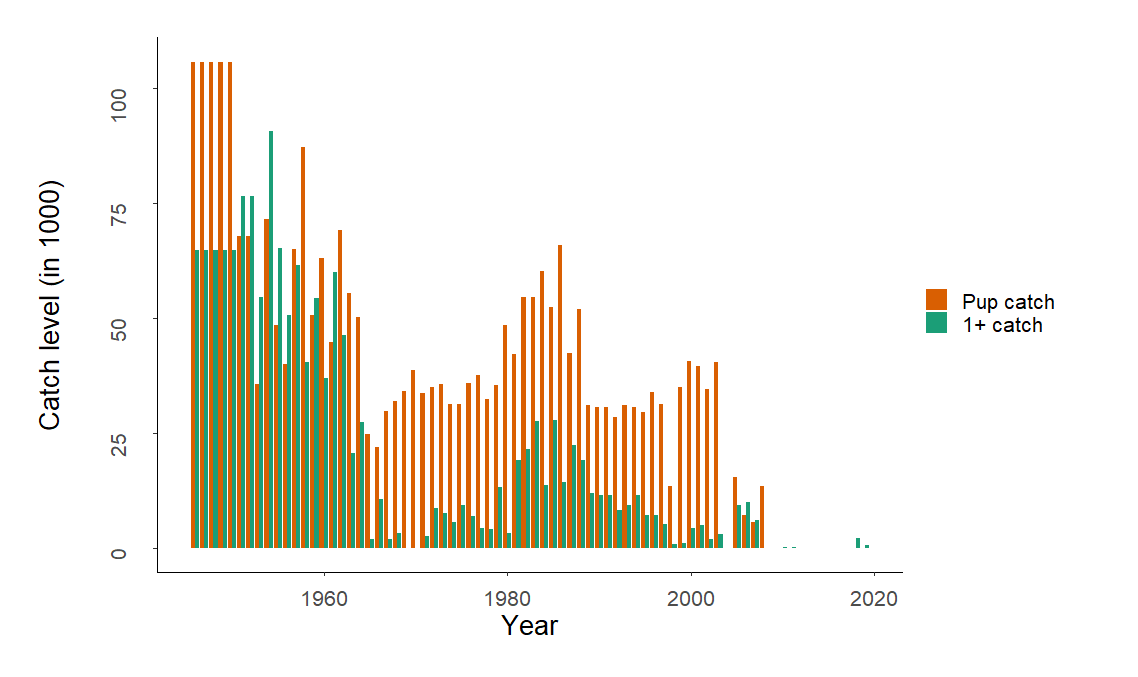
\includegraphics[width=0.98\textwidth,height=\textheight]{figures/catch_data_dodge_new.png}
\caption{Reported catch levels of pups and 1+ animals with bars next to
each other.}
\end{figure}

\begin{center}\rule{0.5\linewidth}{0.5pt}\end{center}

Default the bars are next to each other, but the bars can be plotted on
top of each other by setting \texttt{position\ =\ "stack"}:

\begin{Shaded}
\begin{Highlighting}[]
\KeywordTok{plotCatch}\NormalTok{(}\DataTypeTok{catch =}\NormalTok{ data}\OperatorTok{$}\NormalTok{Cdata,}\DataTypeTok{position =} \StringTok{"stack"}\NormalTok{)}
\end{Highlighting}
\end{Shaded}

\begin{figure}
\centering
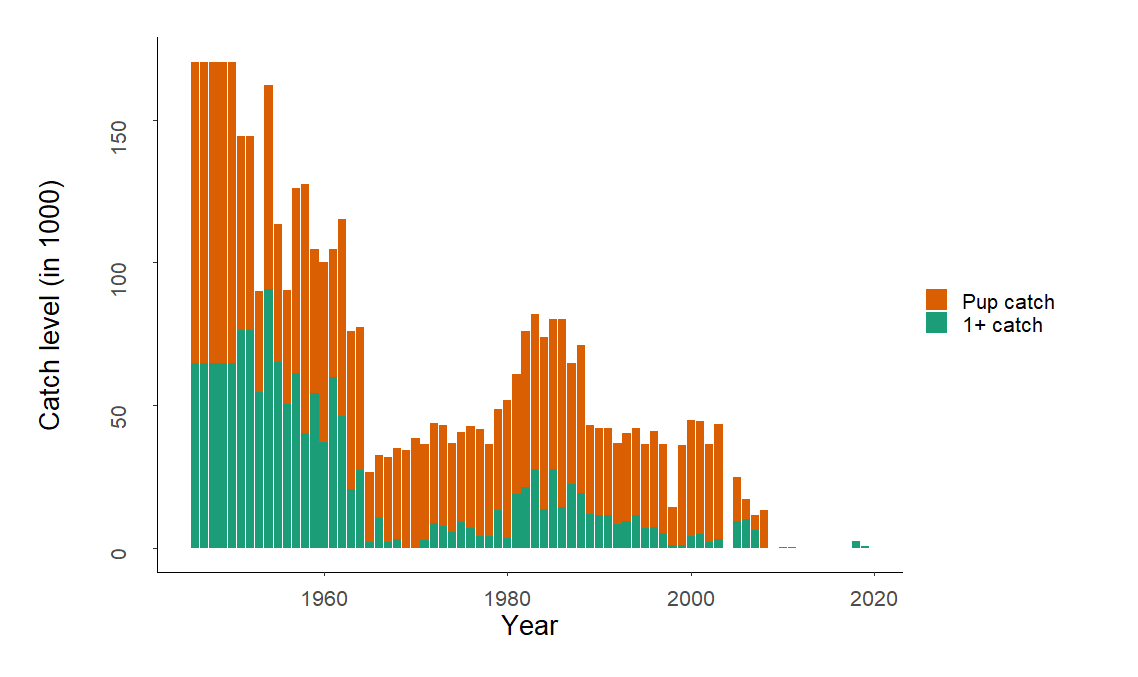
\includegraphics[width=0.98\textwidth,height=\textheight]{figures/catch_data_stack_new.png}
\caption{Reported catch levels of pups and 1+ animals with bars on top
of each other.}
\end{figure}

\begin{center}\rule{0.5\linewidth}{0.5pt}\end{center}

You can plot the modelled population dynamics (pup abundance and total
abundance, not the 1+ population) and the reported catch in the same
figure using \texttt{plotResCatch()}

\begin{Shaded}
\begin{Highlighting}[]
\KeywordTok{plotResCatch}\NormalTok{(res,data)}
\end{Highlighting}
\end{Shaded}

\begin{figure}
\centering
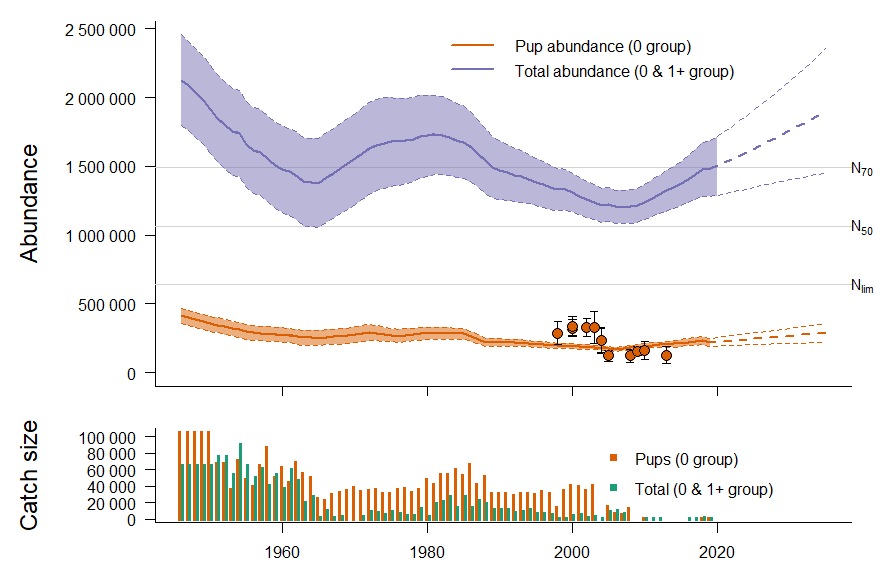
\includegraphics[width=0.98\textwidth,height=\textheight]{figures/plotResCatch2.png}
\caption{Reported catch levels of pups and 1+ animals with bars next to
each other.}
\end{figure}

\begin{center}\rule{0.5\linewidth}{0.5pt}\end{center}

If you want to explore the birth ogive data used for various periods you
can run the \texttt{plotOgive()} function:

\begin{Shaded}
\begin{Highlighting}[]
\KeywordTok{plotOgive}\NormalTok{(}\DataTypeTok{dat =}\NormalTok{ data)}
\end{Highlighting}
\end{Shaded}

\includegraphics{howToUse_rSPAMM_files/figure-latex/unnamed-chunk-26-1.pdf}

\begin{center}\rule{0.5\linewidth}{0.5pt}\end{center}

Since fecundity rates is not available for all years they are
interpolated between missing years. You can plot the fecundity rates
used in the modelling by running \texttt{plotFecundity()}. Default it
plots both the linear interpolated fecundity rates and the observed
fecundity ratesfor a given population.

\begin{Shaded}
\begin{Highlighting}[]
\KeywordTok{plotFecundity}\NormalTok{(}\DataTypeTok{dat =}\NormalTok{ data)}
\end{Highlighting}
\end{Shaded}

\includegraphics{howToUse_rSPAMM_files/figure-latex/unnamed-chunk-27-1.pdf}

\begin{center}\rule{0.5\linewidth}{0.5pt}\end{center}

\hypertarget{exploring-various-catch-options}{%
\section{Exploring various catch
options}\label{exploring-various-catch-options}}

In this section we will describe how to explore various catch options
such as finding the equilibrium catch level, i.e., the fixed annual
catch level that keeps the future projected population abundance
constant, finding the catch level that would reduce the population to
\(N_{70}\) (70\% of the current population size) with probability 0.8
over a 15-years period, and Potential Biological Removals (PBR) catch
level.

\hypertarget{equilibrium-catch-level}{%
\subsection{Equilibrium catch level}\label{equilibrium-catch-level}}

To find the equilibrium catch level we run the function
\texttt{find.eq.quota()}.

Default is that the function assumes that zero pups are in the catch and
that all catch are 1 year old animals or more. To change he proportion
of pups and 1+ animals in the catch you use the \texttt{quota} variable,
i.e., the following finds the equilibrium catch level assuming 15\% pups
and 85\% 1+ animals in the catch:

\begin{Shaded}
\begin{Highlighting}[]
\NormalTok{EquilibriumCatch <-}\StringTok{ }\KeywordTok{find.eq.quota}\NormalTok{(}\DataTypeTok{data =}\NormalTok{ data,}
                                  \DataTypeTok{parameters =}\NormalTok{ parameters, }
                                  \DataTypeTok{quota =} \KeywordTok{c}\NormalTok{(}\FloatTok{0.15}\NormalTok{,}\FloatTok{0.85}\NormalTok{))}
\CommentTok{#> -----------------------------------------------------}
\CommentTok{#> }
\CommentTok{#> Estimated equilibrium:}
\CommentTok{#> Pups:   3440 }
\CommentTok{#> Adults: 19492 }
\CommentTok{#> Total : 22932 }
\CommentTok{#> }
\CommentTok{#> -----------------------------------------------------}

\NormalTok{EquilibriumCatch}
\CommentTok{#> [1]  3439.723 19491.766}
\end{Highlighting}
\end{Shaded}

You have now found the fixed annual catch level that stabilizes the
future 1+ population under the estimated model for the \texttt{harpeast}
population and can re-run the model using this equilibrium catch level
for the future projection. Default in the when running the model fit
assumes zero catch for the future predictions. To re-run the model and
plot the estimated future trajectory using the equilibrium catch level
you run the following code:

\begin{Shaded}
\begin{Highlighting}[]
\CommentTok{#Rerun the model}
\NormalTok{data}\OperatorTok{$}\NormalTok{CQuota =}\StringTok{ }\NormalTok{EquilibriumCatch}
\NormalTok{optEq =}\StringTok{ }\KeywordTok{run.model}\NormalTok{(}\DataTypeTok{data =}\NormalTok{ data, }\DataTypeTok{par =}\NormalTok{ parameters)}
\CommentTok{#> }
\CommentTok{#> --------------------------------------------------}
\CommentTok{#> }
\CommentTok{#>  Optimization converged:  relative convergence (4) }
\CommentTok{#> }
\CommentTok{#> }
\CommentTok{#>  Parameter estimates}
\CommentTok{#>  -------------------}
\CommentTok{#>  Initial population size: K =  1710731 }
\CommentTok{#>  Pup mortality:          M0 =  0.27 }
\CommentTok{#>  1+ mortality:            M =  0.13 }
\CommentTok{#> }
\CommentTok{#> --------------------------------------------------}
\NormalTok{resEq =}\StringTok{ }\KeywordTok{model.results}\NormalTok{(}\DataTypeTok{data =}\NormalTok{ data,}\DataTypeTok{optobject =}\NormalTok{ optEq)}

\CommentTok{#Plot model}
\KeywordTok{plotRes}\NormalTok{(resEq,data)}
\end{Highlighting}
\end{Shaded}

\includegraphics{howToUse_rSPAMM_files/figure-latex/unnamed-chunk-29-1.pdf}

\begin{center}\rule{0.5\linewidth}{0.5pt}\end{center}

\hypertarget{n_70-catch-level}{%
\subsection{\texorpdfstring{\(N_{70}\) catch
level}{N\_\{70\} catch level}}\label{n_70-catch-level}}

To find the the catch level that would reduce the population to 70\% of
the historical maximum observed (modelled) with probability 0.8 over a
15-year period you run the function \texttt{find.N70.quota()}:

\begin{Shaded}
\begin{Highlighting}[]
\NormalTok{catchN70 =}\StringTok{ }\KeywordTok{find.N70.quota}\NormalTok{(}\DataTypeTok{data =}\NormalTok{ data,}
                          \DataTypeTok{parameters =}\NormalTok{ parameters, }
                          \DataTypeTok{quota =} \KeywordTok{c}\NormalTok{(}\DecValTok{0}\NormalTok{,}\DecValTok{1}\NormalTok{))}
\CommentTok{#> }
\CommentTok{#>  ---------------------------------------}
\CommentTok{#> }
\CommentTok{#>  Current population size is already within}
\CommentTok{#>  the 80 percent confidence interval of}
\CommentTok{#>  the  15  year prediction.}
\CommentTok{#>  Hence, no catch level will be estimated.}
\CommentTok{#> }
\CommentTok{#>  ---------------------------------------}
\end{Highlighting}
\end{Shaded}

For this population it turns out that the current population size is
below \(N_{70}\). Because of this there is no point estimating the
\(N_{70}\) catch level.

This example assume that zero pups are in the catch and that all catch
are 1 year old animals or more. To change he proportion of pups and 1+
animals in the catch you use the \texttt{quota} variable, i.e., use
\texttt{quota\ =\ c(0.15,0.85)} to find the \(N{70}\) catch level
assuming 15\% pups and 85\% 1+ animals in the catch:

If the \(N_{70}\) population size was below the current population size
you could re-run the model using the estimated \(N_{70}\) catch level

\begin{Shaded}
\begin{Highlighting}[]
\NormalTok{data}\OperatorTok{$}\NormalTok{CQuota =}\StringTok{ }\NormalTok{catchN70}
\NormalTok{optN70 =}\StringTok{ }\KeywordTok{run.model}\NormalTok{(}\DataTypeTok{data =}\NormalTok{ data, }\DataTypeTok{par =}\NormalTok{ parameters)}
\NormalTok{resN70 =}\StringTok{ }\KeywordTok{model.results}\NormalTok{(}\DataTypeTok{data =}\NormalTok{ data,}\DataTypeTok{optobject =}\NormalTok{ optN70)}

\CommentTok{#Plot the estimated future trajectory using the N70 catch level}
\KeywordTok{plotRes}\NormalTok{(resN70,data)}
\end{Highlighting}
\end{Shaded}

\hypertarget{the-potential-biological-removals-pbr-catch-level}{%
\subsection{The Potential Biological Removals (PBR) catch
level}\label{the-potential-biological-removals-pbr-catch-level}}

Potential Biological Removals has been defined as:
\[PBR=\frac{1}{2}R_{max}F_rN_{min},\] where \(R_{max}\) is the maximum
rate of increase for the population (default to 0.12 for pinnipeds),
\(F_r\) is the recovery factor with values between 0.1 and 1 (default to
0.5), and \(N_{min}\) is the estimated population size using 20\%
percentile of the log-normal distribution. The PBR catch level assumes
that the age structure of the removals is proportional to the age
composition of the population (i.e.~14\% ). To find the PBR catch level
using the default parameters you run:

\begin{Shaded}
\begin{Highlighting}[]
\NormalTok{pbrCatch =}\StringTok{ }\KeywordTok{PBR}\NormalTok{(}\DataTypeTok{n0=}\NormalTok{partab[}\DecValTok{4}\NormalTok{,}\DecValTok{3}\NormalTok{], }
               \DataTypeTok{n1=}\NormalTok{partab[}\DecValTok{5}\NormalTok{,}\DecValTok{3}\NormalTok{], }
               \DataTypeTok{se0=}\NormalTok{partab[}\DecValTok{4}\NormalTok{,}\DecValTok{4}\NormalTok{], }
               \DataTypeTok{se1=}\NormalTok{partab[}\DecValTok{5}\NormalTok{,}\DecValTok{4}\NormalTok{])}

\NormalTok{pbrCatch}
\CommentTok{#> $Nmin}
\CommentTok{#> [1] 1402092}
\CommentTok{#> }
\CommentTok{#> $CV}
\CommentTok{#> [1] 0.07031021}
\CommentTok{#> }
\CommentTok{#> $PBR}
\CommentTok{#> [1] 42063}
\CommentTok{#> }
\CommentTok{#> $n0catch}
\CommentTok{#> [1] 5889}
\CommentTok{#> }
\CommentTok{#> $n1catch}
\CommentTok{#> [1] 36174}
\end{Highlighting}
\end{Shaded}

where n0 is the current population size, n1 is the current 1+ population
size, se0 is the standard deviation of the estimated current pup
abundance, and se1 is the standard deviation of the estimated current 1+
abundance. Recall from the Table above that these quantities could be
found using the \texttt{par.tab()} function.

Re-run the model using this catch level

\begin{Shaded}
\begin{Highlighting}[]
\NormalTok{data}\OperatorTok{$}\NormalTok{Quota =}\StringTok{ }\KeywordTok{c}\NormalTok{(pbrCatch}\OperatorTok{$}\NormalTok{n0catch,pbrCatch}\OperatorTok{$}\NormalTok{n1catch)}
\NormalTok{optPBR =}\StringTok{ }\KeywordTok{run.model}\NormalTok{(}\DataTypeTok{data =}\NormalTok{ data, }\DataTypeTok{par =}\NormalTok{ parameters)}
\CommentTok{#> }
\CommentTok{#> --------------------------------------------------}
\CommentTok{#> }
\CommentTok{#>  Optimization converged:  relative convergence (4) }
\CommentTok{#> }
\CommentTok{#> }
\CommentTok{#>  Parameter estimates}
\CommentTok{#>  -------------------}
\CommentTok{#>  Initial population size: K =  1710731 }
\CommentTok{#>  Pup mortality:          M0 =  0.27 }
\CommentTok{#>  1+ mortality:            M =  0.13 }
\CommentTok{#> }
\CommentTok{#> --------------------------------------------------}
\NormalTok{resPBR =}\StringTok{ }\KeywordTok{model.results}\NormalTok{(}\DataTypeTok{data =}\NormalTok{ data,}\DataTypeTok{optobject =}\NormalTok{ optPBR)}

\CommentTok{#Plot the estimated future trajectory using PBR catch level}
\KeywordTok{plotRes}\NormalTok{(resPBR,data)}
\end{Highlighting}
\end{Shaded}

\includegraphics{howToUse_rSPAMM_files/figure-latex/unnamed-chunk-33-1.pdf}

\begin{center}\rule{0.5\linewidth}{0.5pt}\end{center}

\hypertarget{appendix}{%
\section{Appendix}\label{appendix}}

\hypertarget{complete-code-for-assessment}{%
\subsection{Complete code for
assessment}\label{complete-code-for-assessment}}

This section contains a script for a complete analysis of the harp seal
population in the East Ice (in the White Sea) using the \texttt{rSPAMM}
package.

\begin{Shaded}
\begin{Highlighting}[]
\CommentTok{#Load the rSPAMM package}
\KeywordTok{library}\NormalTok{(rSPAMM)}

\CommentTok{###################}
\CommentTok{# Data}
\CommentTok{###################}
\CommentTok{# You can choose to use either the demo data which is }
\CommentTok{# included in the rSPAMM package or loading the full data}

\CommentTok{#Use this if analysing the demo data.}
\CommentTok{#Loading demo data and parameters}
\KeywordTok{data}\NormalTok{(}\StringTok{"harpeastDemo"}\NormalTok{)}
\NormalTok{data =}\StringTok{ }\NormalTok{harpeast}\OperatorTok{$}\NormalTok{data}
\NormalTok{parameters =}\StringTok{ }\NormalTok{harpeast}\OperatorTok{$}\NormalTok{parameters}


\CommentTok{#Use this if analysing latest version of the}
\CommentTok{#complete data set}
\CommentTok{#Download full data. Default the function will}
\CommentTok{#ask to create a new folder. If you already have }
\CommentTok{#a folder you can add the option }
\CommentTok{#"chooseFolder = FALSE".}
\CommentTok{#Note the Working Directory has to be set to the}
\CommentTok{#root folder of the downloaded data, i.e., not }
\CommentTok{#the Data or the Scripts folder.}
\KeywordTok{downloadData}\NormalTok{()}
\CommentTok{#Loading the data}
\NormalTok{data =}\StringTok{ }\KeywordTok{load.data}\NormalTok{(}\DataTypeTok{population =} \StringTok{"harpeast"}\NormalTok{)}
\CommentTok{#Loading the parameters}
\NormalTok{parameters =}\StringTok{ }\KeywordTok{load.initial.values}\NormalTok{(}\DataTypeTok{population =} \StringTok{"harpeast"}\NormalTok{)}


\CommentTok{##################}
\CommentTok{# Model fitting}
\CommentTok{##################}
\CommentTok{#Run the model}
\NormalTok{optobj =}\StringTok{ }\KeywordTok{run.model}\NormalTok{(}\DataTypeTok{data =}\NormalTok{ data, }\DataTypeTok{par =}\NormalTok{ parameters)}

\CommentTok{#Obtain the results}
\NormalTok{res =}\StringTok{ }\KeywordTok{model.results}\NormalTok{(}\DataTypeTok{data =}\NormalTok{ data,}\DataTypeTok{optobject =}\NormalTok{ optobj)}

\CommentTok{#Create a nice table with the results}
\NormalTok{partab =}\StringTok{ }\KeywordTok{par.table}\NormalTok{(}\DataTypeTok{results=}\NormalTok{res, }\DataTypeTok{dat=}\NormalTok{data) }

\CommentTok{#Plot the results (both the pup model fit and the N1+ population)}
\KeywordTok{plotRes}\NormalTok{(res,data,}\DataTypeTok{grDev =} \OtherTok{TRUE}\NormalTok{)}


\CommentTok{##################}
\CommentTok{# Catch options}
\CommentTok{##################}

\CommentTok{#Find the equilibrium catch level}
\CommentTok{#In this example we are assuming 15% pups }
\CommentTok{#and 85% 1+ animals in the catch}
\NormalTok{EquilibriumCatch =}\StringTok{ }\KeywordTok{find.eq.quota}\NormalTok{(}\DataTypeTok{data =}\NormalTok{ data,}
                                 \DataTypeTok{parameters =}\NormalTok{parameters,}
                                 \DataTypeTok{quota =} \KeywordTok{c}\NormalTok{(}\FloatTok{0.15}\NormalTok{,}\FloatTok{0.85}\NormalTok{))}

\CommentTok{#Rerun the model using the estimated equilibrium catch level}
\NormalTok{data}\OperatorTok{$}\NormalTok{CQuota =}\StringTok{ }\NormalTok{EquilibriumCatch}
\NormalTok{optEq =}\StringTok{ }\KeywordTok{run.model}\NormalTok{(}\DataTypeTok{data =}\NormalTok{ data, }\DataTypeTok{par =}\NormalTok{ parameters)}
\NormalTok{resEq =}\StringTok{ }\KeywordTok{model.results}\NormalTok{(}\DataTypeTok{data =}\NormalTok{ data,}\DataTypeTok{optobject =}\NormalTok{ optEq)}

\CommentTok{#Plot the estimated future trajectory using equilibrium catch level}
\KeywordTok{plotRes}\NormalTok{(resEq,data,}\DataTypeTok{grDev =} \OtherTok{TRUE}\NormalTok{)}

\CommentTok{#--------------------------}

\CommentTok{#Find the N70 catch level}
\NormalTok{catchN70 =}\StringTok{ }\KeywordTok{find.N70.quota}\NormalTok{(}\DataTypeTok{data =}\NormalTok{ data,}
                          \DataTypeTok{parameters =}\NormalTok{ parameters, }
                          \DataTypeTok{quota =} \KeywordTok{c}\NormalTok{(}\DecValTok{0}\NormalTok{,}\DecValTok{1}\NormalTok{))}

\CommentTok{#For this population it turns out that the current population}
\CommentTok{#size is below N70. Because of this there is no point estimating}
\CommentTok{#the N70 catch level.}

\CommentTok{#If the current population size was above N70 you could}
\CommentTok{#rerun the model using the estimated N70 catch level}
\NormalTok{data}\OperatorTok{$}\NormalTok{CQuota =}\StringTok{ }\NormalTok{catchN70}
\NormalTok{optN70 =}\StringTok{ }\KeywordTok{run.model}\NormalTok{(}\DataTypeTok{data =}\NormalTok{ data, }\DataTypeTok{par =}\NormalTok{ parameters)}
\NormalTok{resN70 =}\StringTok{ }\KeywordTok{model.results}\NormalTok{(}\DataTypeTok{data =}\NormalTok{ data,}\DataTypeTok{optobject =}\NormalTok{ optN70)}

\CommentTok{#Plot the estimated future trajectory using the N70 catch level}
\KeywordTok{plotRes}\NormalTok{(resN70,data,}\DataTypeTok{grDev =} \OtherTok{TRUE}\NormalTok{)}

\CommentTok{#--------------------------}

\CommentTok{#Find the PBR catch level}
\CommentTok{#In this example we are assuming 14% pups }
\CommentTok{#and 86% 1+ animals in the catch}
\NormalTok{pbrCatch =}\StringTok{ }\KeywordTok{PBR}\NormalTok{(}\DataTypeTok{n0=}\NormalTok{partab[}\DecValTok{4}\NormalTok{,}\DecValTok{3}\NormalTok{], }
               \DataTypeTok{n1=}\NormalTok{partab[}\DecValTok{5}\NormalTok{,}\DecValTok{3}\NormalTok{], }
               \DataTypeTok{se0=}\NormalTok{partab[}\DecValTok{4}\NormalTok{,}\DecValTok{4}\NormalTok{], }
               \DataTypeTok{se1=}\NormalTok{partab[}\DecValTok{5}\NormalTok{,}\DecValTok{4}\NormalTok{])}

\CommentTok{#Re-run the model using the PBR catch level}
\NormalTok{data}\OperatorTok{$}\NormalTok{CQuota =}\StringTok{ }\KeywordTok{c}\NormalTok{(pbrCatch}\OperatorTok{$}\NormalTok{n0catch,pbrCatch}\OperatorTok{$}\NormalTok{n1catch)}
\NormalTok{optPBR =}\StringTok{ }\KeywordTok{run.model}\NormalTok{(}\DataTypeTok{data =}\NormalTok{ data, }\DataTypeTok{par =}\NormalTok{ parameters)}
\NormalTok{resPBR =}\StringTok{ }\KeywordTok{model.results}\NormalTok{(}\DataTypeTok{data =}\NormalTok{ data,}\DataTypeTok{optobject =}\NormalTok{ optPBR)}

\CommentTok{#Plot the estimated future trajectory using PBR catch level}
\KeywordTok{plotRes}\NormalTok{(resPBR,data,}\DataTypeTok{grDev =} \OtherTok{TRUE}\NormalTok{)}
\end{Highlighting}
\end{Shaded}

\hypertarget{the-population-dynamics-model}{%
\subsection{The population dynamics
model}\label{the-population-dynamics-model}}

The population model is an age-structured population dynamics model. For
initiation of the model it is assumed that the population had a stable
age structure in year \(y_0 = 1945\), i.e., \[
N_{i,y_0} = N_{y_0}s_{1+}^{i-1}(1-s_{1+}), \quad i = 1,\ldots,A-1,
\] \[
N_{A,y_0}=N_{y_0}s_{1+}^{A-1}.
\] Here \(A\) is the maximum age group containing seals aged \(A\) and
higher, and set to 20 years, and \(N_{y_0}\) is the estimated initial
population size in year \(y_0\). The model is parameterized by the
natural mortalities \(M_0\) and \(M_{1+}\) for the pups and seals of 1
year and older, respectively. These mortalities determine the survival
probabilities \(s_0 = \exp(-M_0)\) and \(s_{1+} = \exp(-M_{1+})\).

The model has the following set of recursion equations: \[
N_{a,y}=\left(N_{0,y-1}-C_{0,y-1}\right)s_0,
\] \[
N_{a,y}=\left(N_{a-1,y-1}-C_{a-1,y-1}\right)s_{1+},\quad a=2,\ldots,A-1,
\] \[
N_{A,y}=\left[\left(N_{A-1,y-1}-C_{a-1,y-1}\right)+\left(N_{A,y-1}-C_{A,y-1}\right)\right]s_{1+}.
\] Since available data do not allow for more detailed age-dependence in
survival to be estimated it is assumed that the mortality rates are
age-independent within the 1+ group. The \(C_{a,y}\) are the
age-specific catch numbers. Catch records are aggregated over age, and
only provide information about the annual number of pups and number of
1+ seals caught. To obtain \(C_{a,y}\) we assume that the
age-distribution in the catch follows the modelled age distribution and
employ \emph{pro rata} rules in the model: \[
C_{a,y} = C_{1+,y}\frac{N_{a,y}}{N_{1+,y}},\quad a = 1,\ldots,A.
\]

where \(N_{1+,y} = \sum_{y=1}^A N_{a,y}\), with \(N_{a,y}\) being the
number of individuals ate age \(a\) in year \(y\).

The modelled pup abundance is given by \[
N_{0,y}=\frac{F_y}{2}\sum_{a=1}^Ap_{a,y}N_{a.y},
\]

where \(N_{a,y}/2\) is the number of females ate age \(a\) in year
\(y\), \(F_y\) is the time-varying fecundity rates and \(p_{a,y}\) are
the time-varying age specific proportions of mature females.

The model is fitted to the survey pup production estimates and the
fecundity rates by maximum likelihood. Assuming normality for the pup
production estimates, their contribution to the log-likelihood function
is \[
\sum_y-\log(\sigma_{0,y})-\frac{1}{2}\frac{\left(N_{0,y}-n_{0,y}\right)^2}{\left(\sigma_{0,y}\right)^2},
\] where \(n_{0,y}\) and \(\sigma_{0,y}\) denote the survey pup
production count and corresponding standard error for year \(y\).

The model has a Bayesian flavour as priors are imposed on some of the
parameters. A vague normal prior is assumed for the initial population
size \(N_{y_0}\). A truncated normal prior was used for both the pup
mortalities \(M_0\) and \(M_{1+}\).

All parameter estimates are found by maximizing the likelihood function
using the R package \texttt{TMB}.

\end{document}
